\documentclass[12pt, a4paper]{article}
\usepackage[utf8]{inputenc}
\usepackage{amsmath}
\usepackage{amsthm}
\usepackage{graphicx}
\usepackage{parskip}
\usepackage{hyperref}
\usepackage{fancyhdr}
\usepackage{lastpage}
\usepackage{tikz}
\usepackage{float}
\usepackage{listings}
\usepackage{color}
\usepackage{caption}
\usepackage[acronym]{glossaries}
\graphicspath{ {./images/} }

\tikzstyle{bag} = [align=center]

\lstset{frame=tb,
  language=Haskell,
  aboveskip=3mm,
  belowskip=3mm,
  showstringspaces=false,
  columns=flexible,
  basicstyle={\small\ttfamily},
  numbers=left,
  numberstyle=\tiny\color{gray},
  keywordstyle=\color{blue},
  commentstyle=\color{dkgreen},
  stringstyle=\color{mauve},
  breaklines=true,
  breakatwhitespace=true,
  tabsize=2,
  stepnumber=1,
  escapechar=!
}

\definecolor{dkgreen}{rgb}{0,0.6,0}
\definecolor{gray}{rgb}{0.5,0.5,0.5}
\definecolor{mauve}{rgb}{0.58,0,0.82}

\title{%
      Homework 1 \\
      Experimental Prove of $\theta(\log n)$ height on Random Binary Search Trees
}
\author{%
  Juan Pablo Royo Sales \\
  \small{Universitat Politècnica de Catalunya}
}
\date\today

\pagestyle{fancy}
\fancyhf{}
\fancyhead[C]{}
\fancyhead[R]{Juan Pablo Royo Sales - UPC MIRI}
\fancyhead[L]{ADS - Homework 1}
\fancyfoot[L,C]{}
\fancyfoot[R]{Page \thepage{} of \pageref{LastPage}}
\setlength{\headheight}{15pt}
\renewcommand{\headrulewidth}{0.4pt}
\renewcommand{\footrulewidth}{0.4pt}

\makeglossaries

\newacronym{bst}{BST}{Binary Search Tree}
\newacronym{rbst}{RandomBST}{Randomly Built Binary Search Tree}
\newacronym{treap}{Treap}{Treap}
\newacronym{rtreap}{RTreap}{Randomized Treap}

\begin{document}

\maketitle

\section{Introduction}
In this Homework I have selected to explore and analyze \textbf{\acrfull{rbst}} in order to prove through experimentation that the expected height of \textit{\acrshort{rbst}} is $E[h] = \theta(\log n)$ as it is formally proved in \cite{cormen}.

In order to do that we are going to first give a brief introduction to this type of Data Structure and the theoretical analysis of this feature.

\section{Randomly Built Binary Search Tree}
A \acrshort{rbst} is a \textbf{\acrfull{bst}} that is specifically built using random insertions, in order to achieve \textbf{balanced} \acrshort{bst} \textit{whp}.

Given an insertion in a \acrshort{rbst} of size $n - 1$ there exists the same probability for the key to be inserted in the same interval that the keys already present in the tree. Basically all $n{!}$ possible permutations of the keys are equally likely.

There exists a specific implementation, which is the one I used to conduct the analysis, which is \textbf{\acrfull{rtreap}}.

In the following sections I am going to describe this Data Structure that fulfill the specification of an \acrshort{rbst}.

\section{Treap and Randomized Treap}
A \textbf{\acrfull{treap}} is a \acrshort{bst} in which every node has both the proper key and a priority associated with it $(k_i, p_i)$, such that the Left subtree $L$ of an specific node $N_i = (k_i, p_i)$ contains keys whose values are less than the parent and priorities are less than the parent $\forall j, j \in L \land j \neq i \implies k_i \geq k_j \land p_i \leq p_j$. On the other hand the right subtree $R$ of $N_i$ contains keys whose values the greater and priorities that are less such that $\forall j, j \in R \land j \neq i \implies k_i \leq k_j \land p_i \leq p_j$. A \acrshort{treap} can be seen as a \acrshort{bst} for the search keys and a min-heap for the priorities.

\begin{figure}[H]
\centering
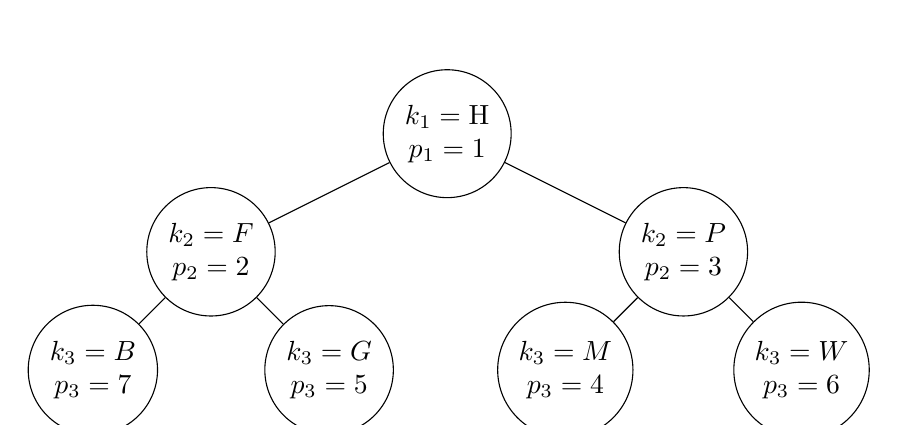
\begin{tikzpicture}[level/.style={sibling distance=60mm/#1}]
  \node [bag,circle,draw](z){
    $k_1 = \text{H}$ \\
    $p_1 = 1$}
    child {node [bag,circle,draw] (a) {$k_2 = F$ \\ $p_2 = 2$}
      child {node [bag,circle,draw] (d) {$k_3 = B$ \\ $p_3 = 7$}}
      child {node [bag,circle,draw] (e) {$k_3 = G$ \\ $p_3 = 5$}}
    }
    child {node [bag,circle,draw] (a) {$k_2 = P$ \\ $p_2 = 3$}
      child {node [bag,circle,draw] (d) {$k_3 = M$ \\ $p_3 = 4$}}
      child {node [bag,circle,draw] (e) {$k_3 = W$ \\ $p_3 = 6$}}
    };
\end{tikzpicture}
\caption{Treap Example} \label{fig:treap_fig_ex}
\end{figure}

\subsection{Operations - Insert}
In order to maintain the Priorities on a new insertion, this data structure requires a \textit{left or right rotation} depending on the priority of the heap that the insertion moment. If we are going to insert a new key $x$, as long as $x$ has a smaller priority than its parent, we perform a rotation on $x$, which basically decrease the \textbf{depth} of $x$ by one and increase parent's depth by one. The rotations are perform in constant time, since it is done with a pointer rotation.

Inserting a new node with key $k$ takes either $O(\text{depth}(p))$ time or $O(\text{depth}(s))$, where $p$ is the predecessor and $s$ is the successor of the new node.

Deletion takes the same time but in the other way around.

\section{Randomized Treap}
A \acrshort{rtreap} it is a \acrshort{treap} that selects the priority of the new insertion node \textit{u.a.r.}.
Given a new key $x$ to be inserted in the \acrshort{rtreap}, a random number is assigned as a priority. In the implementation I have developed for this analysis, I have chosen a big Integer number to be assigned with range $0\ \text{and}\ 2^{31}-1$ but in practice it can be also used a real number between $0$ and $1$. According to the previous definition, because priorities are independent, each node is equally likely to have the smallest priority to be assigned.

The cost of the basics operations of this data structures \textit{search, insert and delete} are proportional to the \textbf{depth} of some node in  the tree. As I have pointed out in the introduction this cost is $\theta(\log n)$ and the prove can be seen here \cite{cormen}.

\section{Experimental Analysis}
In this section I am going to describe the implementation of \acrshort{rbst} I have made and the experiments I run in order to prove that the empirical evidence approximate to the theoretical cost that I have shown previously.

\subsection{Implementation}
I have implemented \acrshort{rbst} in \textbf{Haskell} based on the implementation published in the official Haskell Wiki page \cite{haskell_impl}.

The implementation has 2 parts: the \acrshort{treap} implementation with all the logic and on top of that, taking advantage of the composition abilities that Functional Programming languages have, the implementation of \acrshort{rtreap}.


\begin{lstlisting}[language=Haskell,title={\textbf{RandomBST.hs} - Treap Implementation with Insert function}]

  data Treap k p = Empty | Node (Treap k p) k p (Treap k p)
   deriving (Show, Read)


  tInsert :: (Ord k, Ord p) => k -> p -> Treap k p -> Treap k p
  tInsert k p Empty                     = Node Empty k p Empty
  tInsert k p t@(Node left k' p' right) = case compare k k' of
    EQ -> t
    LT -> case Node (tInsert k p left) k' p' right of
      t'@(Node (Node _ _ p'' _) _ p''' _) ->
        if p''' > p'' then rotateRight t' else t'
      _ -> t
    GT -> case Node left k' p' (tInsert k p right) of
      t'@(Node _ _ p''' (Node _ _ p'' _)) ->
        if p''' > p'' then rotateLeft t' else t'
      _ -> t

  rotateLeft :: Treap k p -> Treap k p
  rotateLeft (Node a k p (Node b1 k' p' b2)) = Node (Node a k p b1) k' p' b2
  rotateLeft _                               = error "Wrong rotation (rotateLeft)"

  rotateRight :: Treap k p -> Treap k p
  rotateRight (Node (Node a1 k' p' a2) k p b) = Node a1 k' p' (Node a2 k p b)
  rotateRight _ = error "Wrong rotation (rotateRight)"

\end{lstlisting}


\begin{lstlisting}[language=Haskell,title={\textbf{RandomBST.hs} - Random Treap Implementation with Insert function compose with underlying Treap}]

  newtype RTreap g k p = RT (g, Treap k p)
   deriving (Show, Read)


  insert
    :: (RandomGen g, Ord k, Bounded p, Ord p, Num p, Random p)
    => k
    -> RTreap g k p
    -> RTreap g k p
  insert k (RT (g, tr)) =
    let (p, g') = randomR (0, maxBound) g in RT (g', tInsert k p tr)

\end{lstlisting}

There are more code that includes helper functions to gather metrics, testing with Property Based Testing in Quickcheck and other helper functions. This can be found with the bundle package and references are in Appendix section.

\subsection{Experiments}
The following are the experiments I have conducted in order to have empirical prove that the tested height approximates to $\log n$.

\begin{itemize}
  \item Generate a random list of $n$ distinct elements
  \item Build a \acrshort{rbst} with the given random list.
\end{itemize}

 \begin{table}[H]
    \begin{tabular}{ |c|c|c| }
      \hline
      \multicolumn{3}{|c|}{Experiments Conducted on Insertion and Deletion in \acrshort{rbst}}\\
      \hline
      Experiment \# & Input Size & Operations \\
      \hline
      1 & 64 & Insertion \\
      2 & 64 & Insertion and Deletion \\
      3 & 128 & Insertion \\
      4 & 128 & Insertion and Deletion \\
      5 & 256 & Insertion \\
      6 & 256 & Insertion and Deletion \\
      7 & 512 & Insertion \\
      8 & 512 & Insertion and Deletion \\
      9 & 1024 & Insertion \\
      10 & 1024 & Insertion and Deletion \\
      11 & 4096 & Insertion \\
      12 & 4096 & Insertion and Deletion \\
      13 & 8192 & Insertion \\
      14 & 8192 & Insertion and Deletion \\
      15 & 9000 & Insertion \\
      16 & 9000 & Insertion and Deletion \\
      17 & 9500 & Insertion \\
      18 & 9500 & Insertion and Deletion \\
      19 & 10000 & Insertion \\
      20 & 10000 & Insertion and Deletion \\
      21 & 12000 & Insertion \\
      22 & 12000 & Insertion and Deletion \\
      23 & 20000 & Insertion \\
      24 & 20000 & Insertion and Deletion \\
      25 & 40000 & Insertion \\
      26 & 40000 & Insertion and Deletion \\
      27 & 60000 & Insertion \\
      28 & 60000 & Insertion and Deletion \\
      29 & 100000 & Insertion \\
      30 & 100000 & Insertion and Deletion \\
      31 & 200000 & Insertion \\
      32 & 200000 & Insertion and Deletion \\
      33 & 500000 & Insertion \\
      34 & 500000 & Insertion and Deletion \\
      35 & 1000000 & Insertion \\
      36 & 1000000 & Insertion and Deletion \\
      37 & 10000000 & Insertion \\
      38 & 10000000 & Insertion and Deletion \\
      \hline
    \end{tabular}
    \captionof{figure}{Experiments Details}
    \label{table:experiments_detail}
  \end{table}


  In the case of the \textit{Operations}, \textbf{Insertion} means that only use \lstinline[language=Haskell]!insert! combinator to build the \acrshort{rbst} base on the input list. On the other hand \textbf{Insertion and Deletion} means do the \textbf{Insertion} operation to build the \acrshort{rbst} based on the input and random deletions with the \lstinline[language=Haskell]!delete! combinator.

\subsection{Results}
After running all the experiments here we have the following results.

\begin{table}[H]
    \begin{tabular}{ |c|c|c|c|c| }
      \hline
      \multicolumn{5}{|c|}{Results Experiments} \\
      \hline
      Experiment \# & Input Size & Exp. Height & Theoretical Height & Avg. Leaf Depth  \\
      \hline
      1 & 64 & 12 & 6 & 7.75384615384615 \\
      2 & 64 & 12 & 6 & 7.734375 \\
      3 & 128 & 13 & 7 & 9.34883720930233 \\
      4 & 128 & 13 & 7 & 9.3359375 \\
      5 & 256 & 16 & 8 & 9.87937743190662 \\
      6 & 256 & 16 & 8 & 9.85546875 \\
      7 & 512 & 21 & 9 & 12.5087719298246 \\
      8 & 512 & 21 & 9 & 12.5 \\
      9 & 1024 & 24 & 10 & 13.5873170731707 \\
      10 & 1024 & 24 & 10 & 13.5859375 \\
      11 & 4096 & 29 & 12 & 15.8525750549182 \\
      12 & 4096 & 29 & 12 & 15.85205078125 \\
      13 & 8192 & 29 & 12.999999 & 17.0411326742341 \\
      14 & 8192 & 29 & 12.999999 & 17.0408935546875 \\
      15 & 9000 & 29 & 13.135709 & 16.9927785801578 \\
      16 & 9000 & 29 & 13.135709 & 16.9923333333333 \\
      17 & 9500 & 29 & 13.213712 & 16.9861067256078 \\
      18 & 9500 & 29 & 13.213712 & 16.9849473684211 \\
      19 & 10000 & 29 & 13.287712 & 17.003799620038 \\
      20 & 10000 & 29 & 13.287712 & 17.0027 \\
      21 & 12000 & 33 & 13.550747 & 17.9501708190984 \\
      22 & 12000 & 33 & 13.550747 & 17.9506666666667 \\
      23 & 20000 & 34 & 14.287712 & 18.5192740362982 \\
      24 & 20000 & 34 & 14.287712 & 18.5189 \\
      25 & 40000 & 35 & 15.287712 & 20.1334216644584 \\
      26 & 40000 & 35 & 15.287712 & 20.133175 \\
      27 & 60000 & 35 & 15.872675 & 19.9277012049799 \\
      28 & 60000 & 35 & 15.872675 & 19.9276833333333 \\
      29 & 100000 & 37 & 16.60964 & 21.0380096199038 \\
      30 & 100000 & 37 & 16.60964 & 21.03796 \\
      31 & 200000 & 42 & 17.60964 & 22.8204208978955 \\
      32 & 200000 & 42 & 17.60964 & 22.82043 \\
      33 & 500000 & 44 & 18.931568 & 24.8563522872954 \\
      34 & 500000 & 44 & 18.931568 & 24.856346 \\
      35 & 1000000 & 49 & 19.931568 & 26.998066001934 \\
      36 & 1000000 & 49 & 19.931568 & 26.998065 \\
      37 & 10000000 & 60 & 23.253496 & 31.704819929518 \\
      38 & 10000000 & 60 & 23.253496 & 31.7048201 \\
      \hline
    \end{tabular}
    \captionof{figure}{Result Experiments}
    \label{table:experiments_results}
  \end{table}



  \begin{minipage}[t]{\linewidth}
    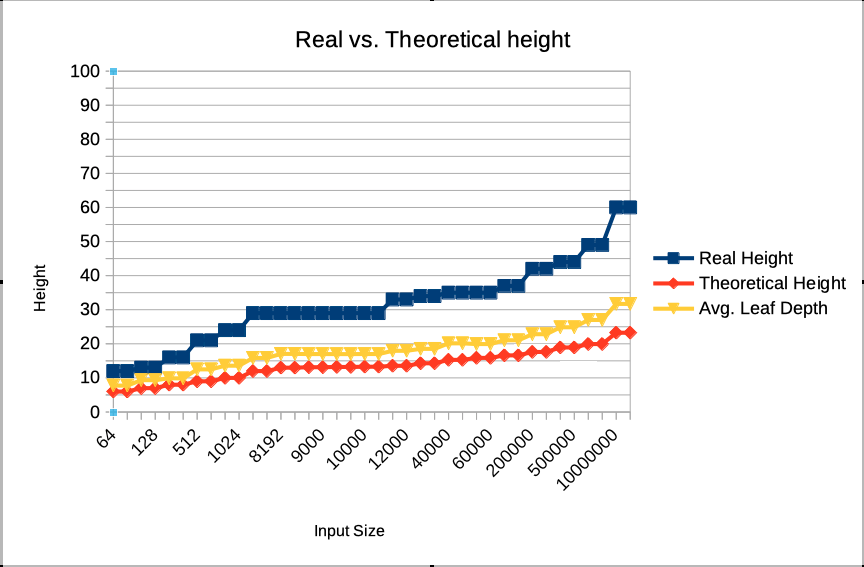
\includegraphics[width=\textwidth]{results}
    \captionof{figure}{Comparison Real vs. Theoretical height and Average Leaf Depth}
    \label{fig:graph_result}
  \end{minipage}

  \textbf{Theoretical Height} means the result of applying $\log_2{n}$ to the input size that we have inserted for that Experiment test case.

\subsubsection{Analysis}
As we can see in \ref{fig:graph_result} the empirical data show us that the height is near the theoretical statement of having a Balanced tree of height $\sim \theta(\log(n))$.

It is true that after a size of $n \geq 1024$ the line increases faster than $\log(n)$ but between $8192$ and $12000$ it stabilized. For large values like $10000000$ it seems it has a peak that goes away from logarithmic function, but it is not unbalanced.

Although we can think that this is a reason to reject the hypothesis with, We can detected that the empirical data doesn't show an unbalanced tree, because of the \textbf{Average Leaf Depth} which proves that for all sizes, the average depth in leafs are logarithmic.

\section{Conclusion}
In conclusion based on the empirical data we can assure that the height of a \acrfull{rbst} is $\theta(\log(n))$.

\appendix
\section{Haskell Code}
I am going to describe how you can run the code, testing and where are source files located.

\subsection{Source Code}
In the source code there are 3 folders with code:

\begin{itemize}
  \item \textbf{app}: Which contains the \textit{Main.hs} which is the entry point of the program to run the experiments.
  \item \textbf{src}: Which contains 2 files \textit{RandomBST.hs} with the \acrshort{rbst} implementation and operations. Also in that folder we have \textit{Experiments.hs} which contains helper functions to run the experiments.
  \item \textbf{test}: Contains the Property Based Testing which allows to test the structure in a random manner.
\end{itemize}

\subsection{Run the Code}
All the solution has been coded with \textbf{Stack} \cite{stack} version 2.1.3 or higher. It is a prerequisite to install \textit{stack} for running this code.

\subsubsection{Running Experiments}

In order to run the experiments just do the following:

\begin{lstlisting}[language=Haskell,title={Running Experiments}]
shell> stack build
shell> stack exec random-bst
\end{lstlisting}


\subsubsection{Running Testing}

In order to run the tests just do the following:

\begin{lstlisting}[language=Haskell,title={Running Experiments}]
shell> stack build
shell> stack test
\end{lstlisting}

\section{Testing Results}


  \begin{minipage}[t]{\linewidth}
    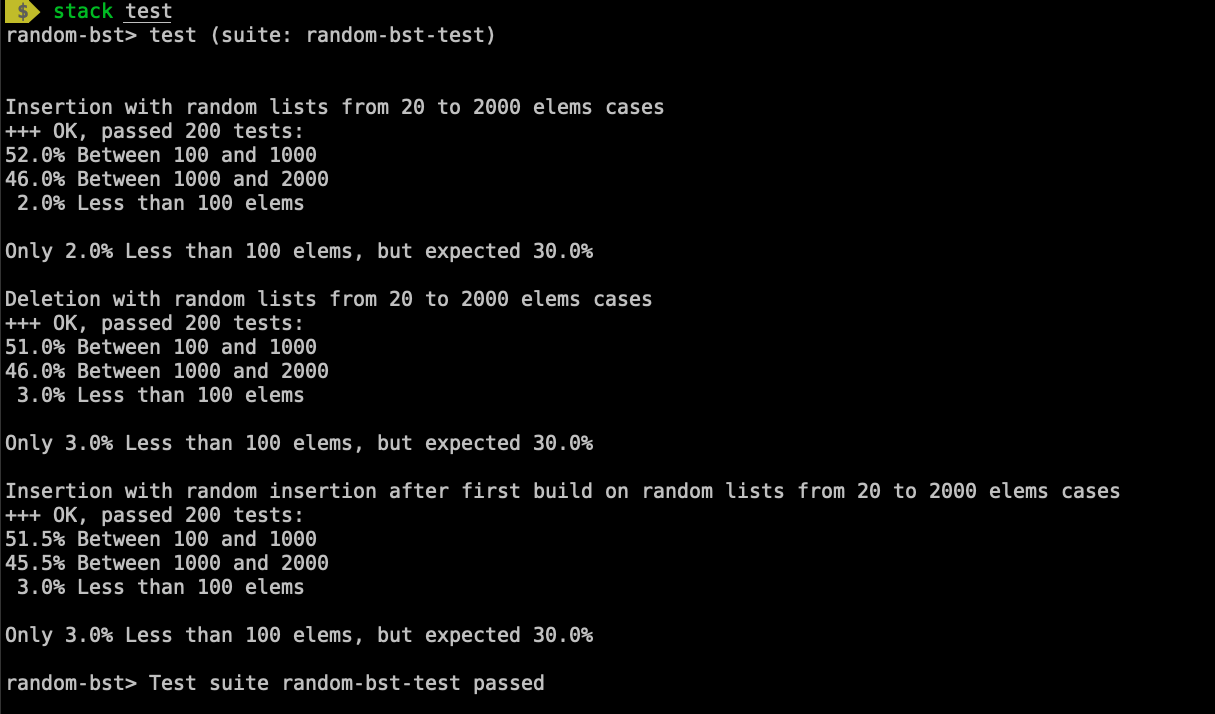
\includegraphics[width=\textwidth]{tests}
    \captionof{figure}{Example of one Testing Result Run}
    \label{fig:test_result}
  \end{minipage}


\printglossary[type=\acronymtype]

\begin{thebibliography}{9}
\bibitem{cormen}
  Cormen, T.H., Stein, C., Rivest, R.L., Leiserson, C.E. 2001. \textit{Introduction to Algorithms}. 2nd edn. McGraw-Hill Higher Education.
\bibitem{haskell_impl}
  Haskell Wiki Issue 4. \url{https://wiki.haskell.org/The_Monad.Reader/Issue4/On_Treaps_And_Randomization}.
\bibitem{stack}
  Stack Tool. \url{https://docs.haskellstack.org/en/stable/README/}
\end{thebibliography}


\end{document}

